\subsection{Distancia promedio recorrida por los usuarios.}

Para calcular la distancia entre estaciones se uso la ecuación \ref{eq:distance}.

\begin{equation}
    \begin{matrix}
        \beta = sin^2\left ( \frac{|\Delta \theta|}{2} \right ) + cos \left (\theta_1\right )  cos(\theta_2)sin^2 \left (\frac{|\Delta \phi|}{2} \right ) \\
        D     = 2R\;arcsin\left (\sqrt{\beta} \right )
    \end{matrix}
    \label{eq:distance}
\end{equation}

donde R es el radio de la tierra, $\theta_i$ es la latitud y $\phi_i$ es la longitud.

En base a eso, se usaron las ecuaciones \ref{eq:monthly_hourly_mean}, \ref{eq:monthly_hourly_var}, \ref{eq:daily_hourly_mean} y \ref{eq:daily_hourly_var}. Los resultados obtenidos son los siguientes:

\subsubsection{Promedio y desviación estandar mensual por hora}

En la figura \ref{fig:monthly_hourly_mean_distance} se visualiza que existe una disminución del uso de las bicicletas entre las 10 y 16 horas a lo largo del año. Además, entre los meses mayo y julio existe una disminución de manera general. Este periodo de meses coincide con la temporada del año donde se presentan con mayor frecuencia lluvias\cite{clima_guadalajara}. Con esto, tenemos que existe un mínimo de la distancia recorrida entre las 14 y 16 horas en los meses de junio y julio. Con ayuda de la figura \ref{fig:monthly_hourly_var_distance} se obtiene que la distancia recorrida por los usuarios entre los meses de septiembre y diciembre tienen una mayor variación y esto puede deberse a la baja temperatura\cite{clima_guadalajara}. Ya que los usuarios al sentir menos presión en sus cuerpos por la temperatura pueden desviarse de sus caminos usuales.

\begin{figure}[H]
    \centering
    \begin{subfigure}[b]{8cm}
        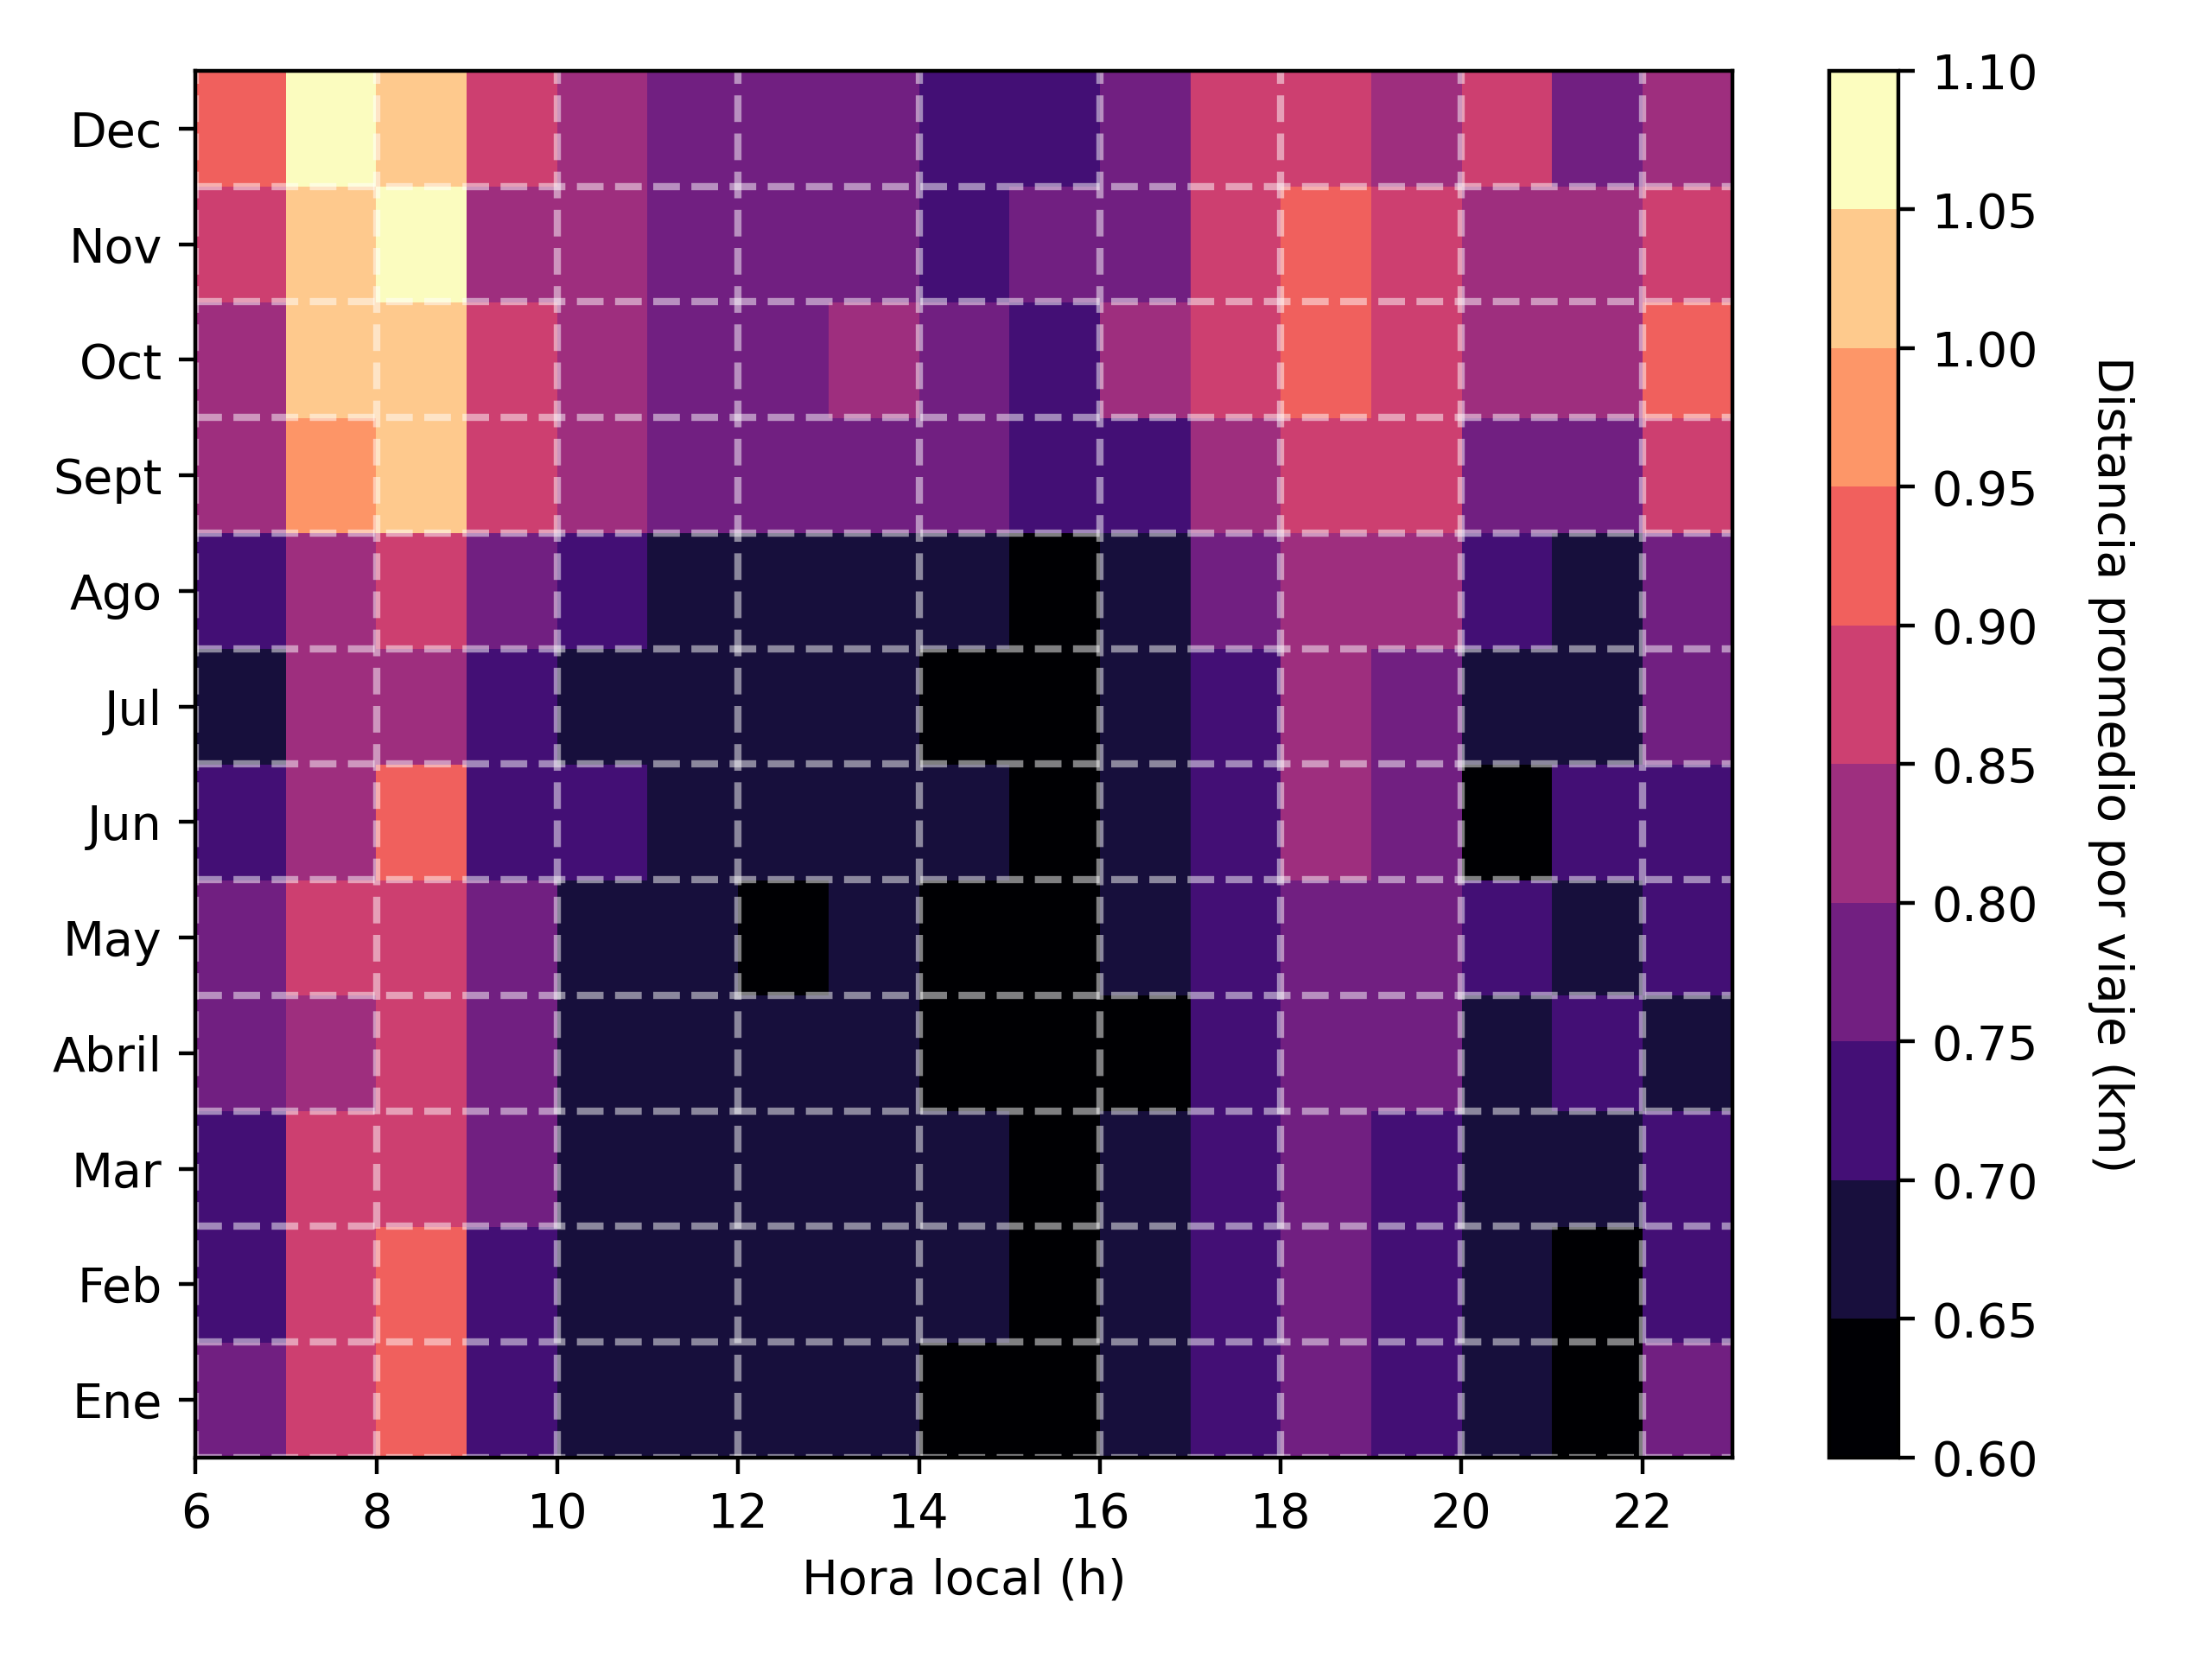
\includegraphics[width=8cm]{Graphics/monthly_hourly_mean_distance.png}
        \caption{Promedio mensual de la distancia recorrida.}
        \label{fig:monthly_hourly_mean_distance}
    \end{subfigure}
    \begin{subfigure}[b]{8.5cm}
        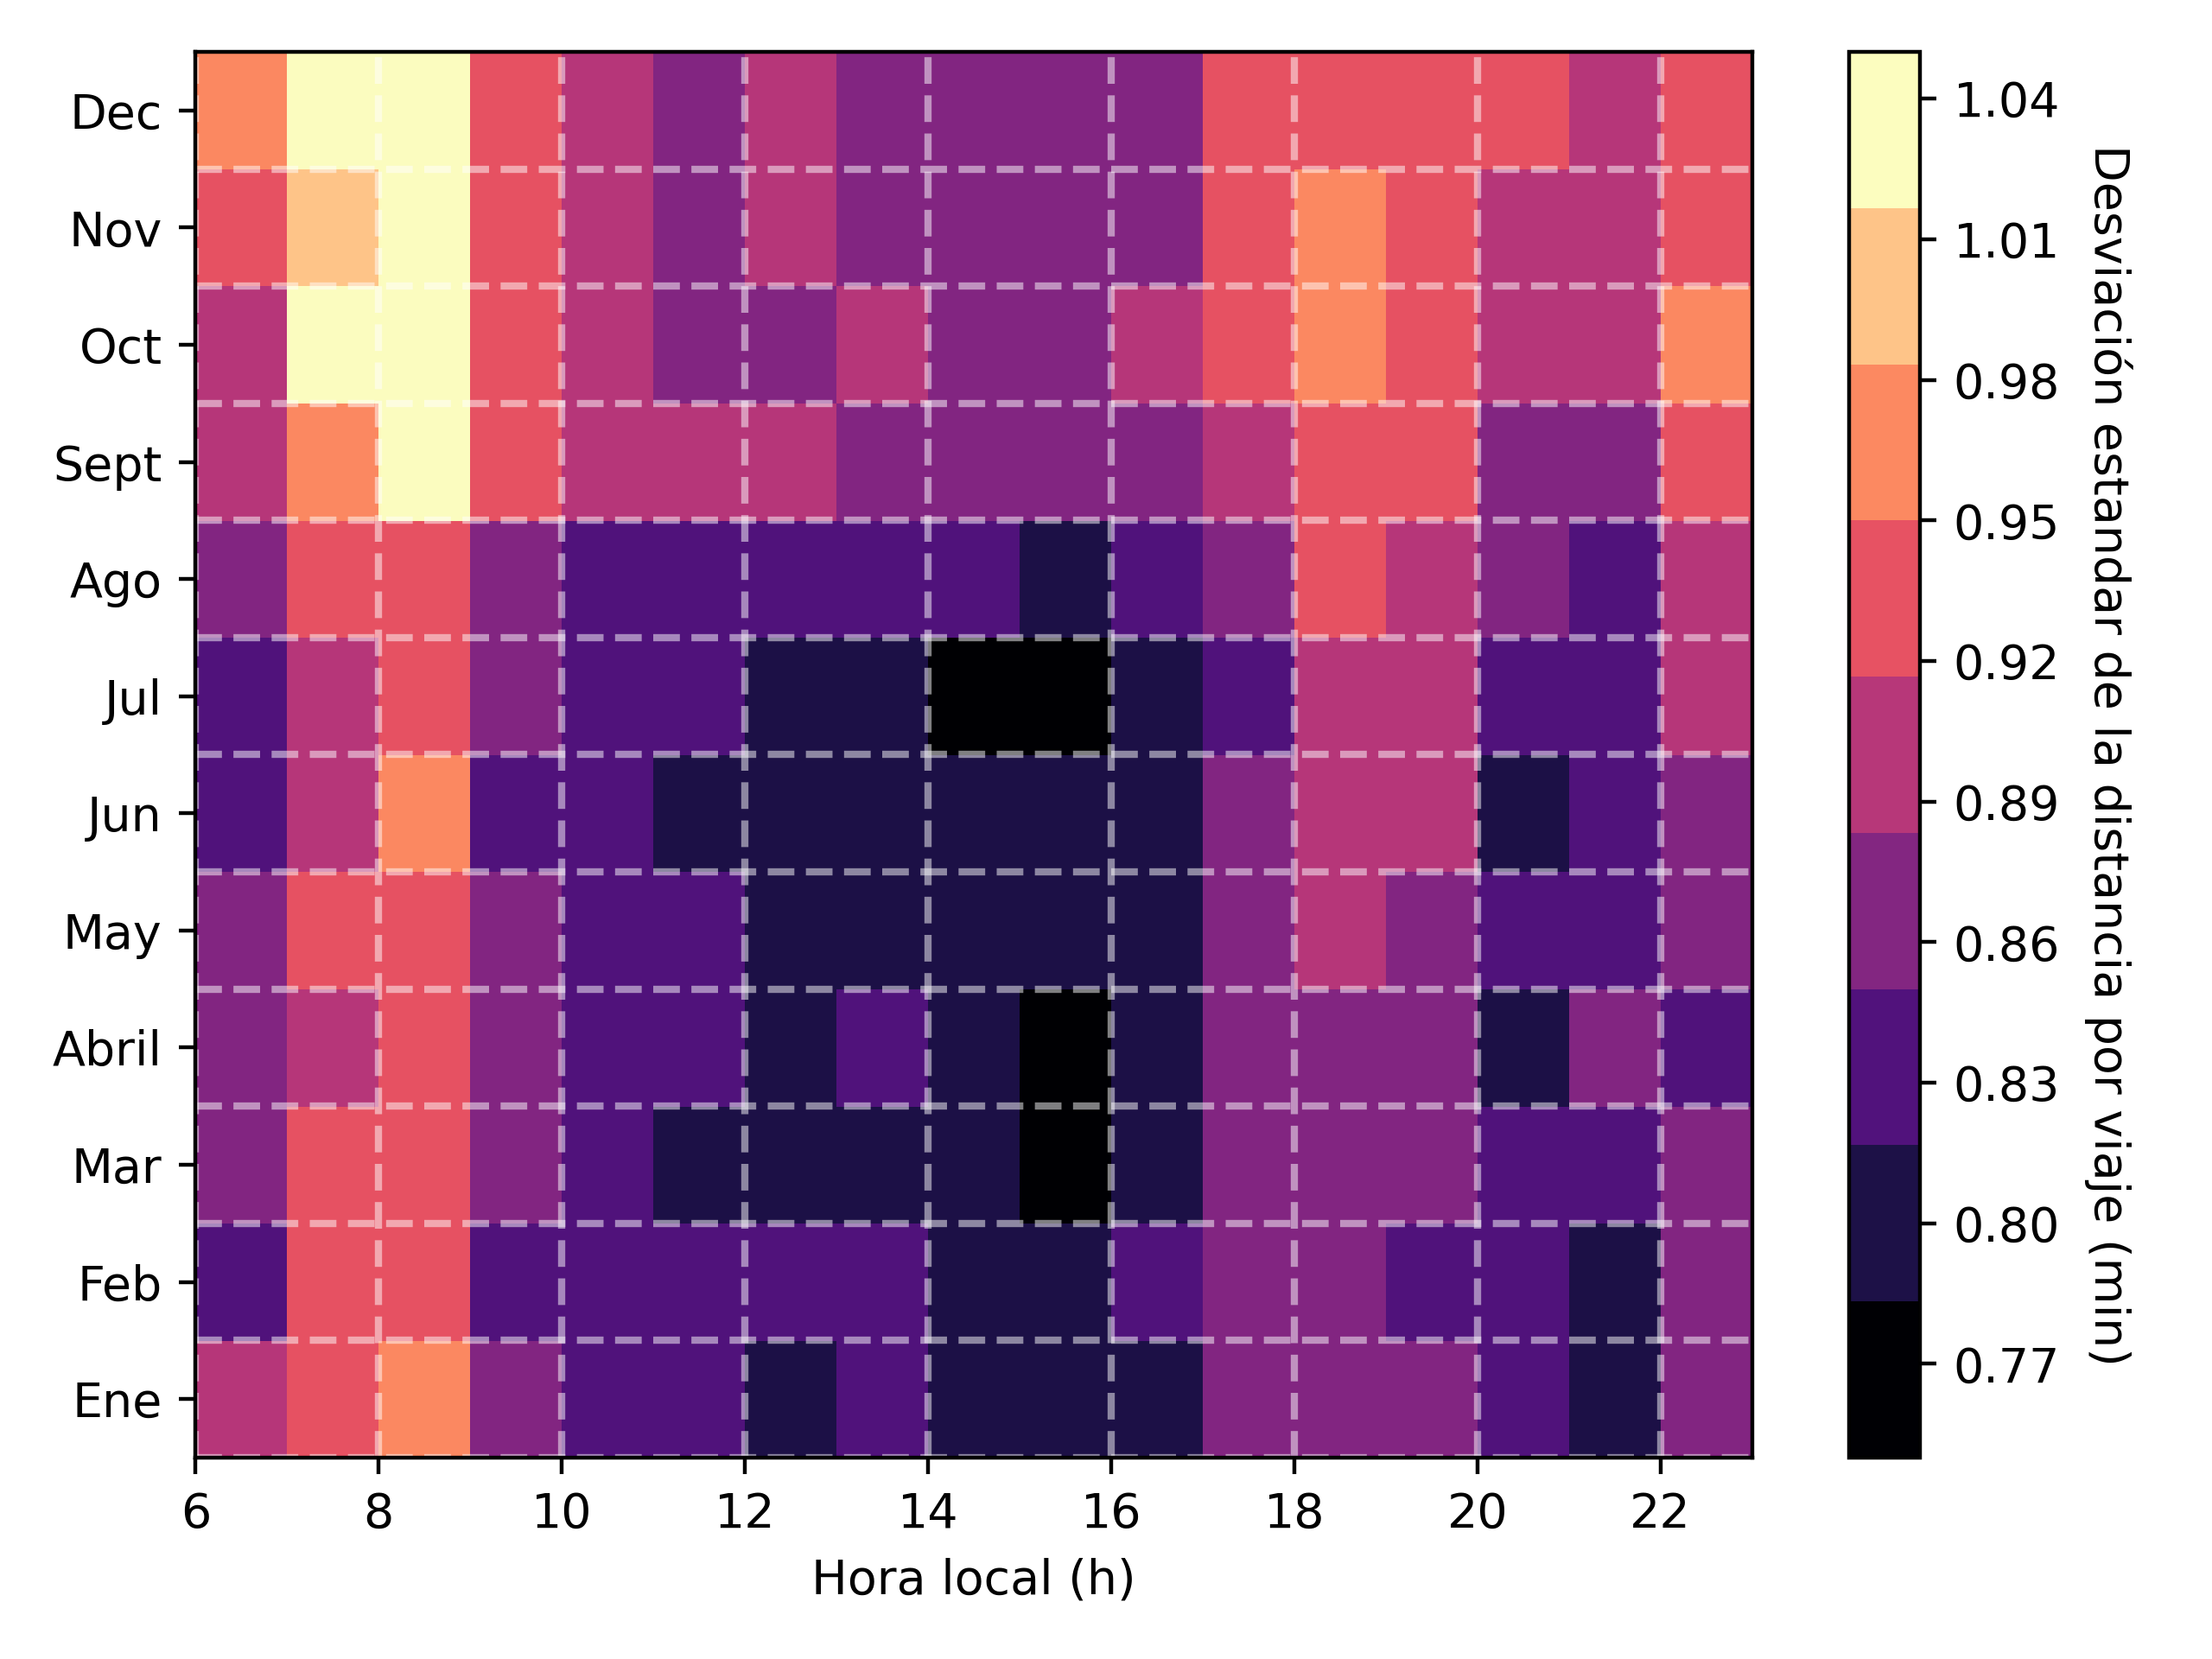
\includegraphics[width=8cm]{Graphics/monthly_hourly_var_distance.png}
        \caption{Desviación estandar de la distancia recorrida.}
        \label{fig:monthly_hourly_var_distance}
    \end{subfigure}
    \caption{Distancia promedio y desviación estandar mensual por hora recorrida por lo usuarios calculadas con las ecuaciones \ref{eq:monthly_hourly_mean} y \ref{eq:monthly_hourly_var}.}
    \label{fig:monthly_hourly_distance}
\end{figure}

\subsubsection{Promedio y desviación estadar diaria semanal por hora}

En la figura \ref{fig:daily_hourly_distance} se aprecia que el uso de la bicicleta se incrementa entre semana a las 7 y 15 horas. Existe una disminución de la distancia recorrida entre las 12 y 16 horas, algo que ya se habia previsto en la figura \ref{fig:daily_hourly_mean_distance}.

\begin{figure}[H]
    \centering
    \begin{subfigure}[b]{8cm}
        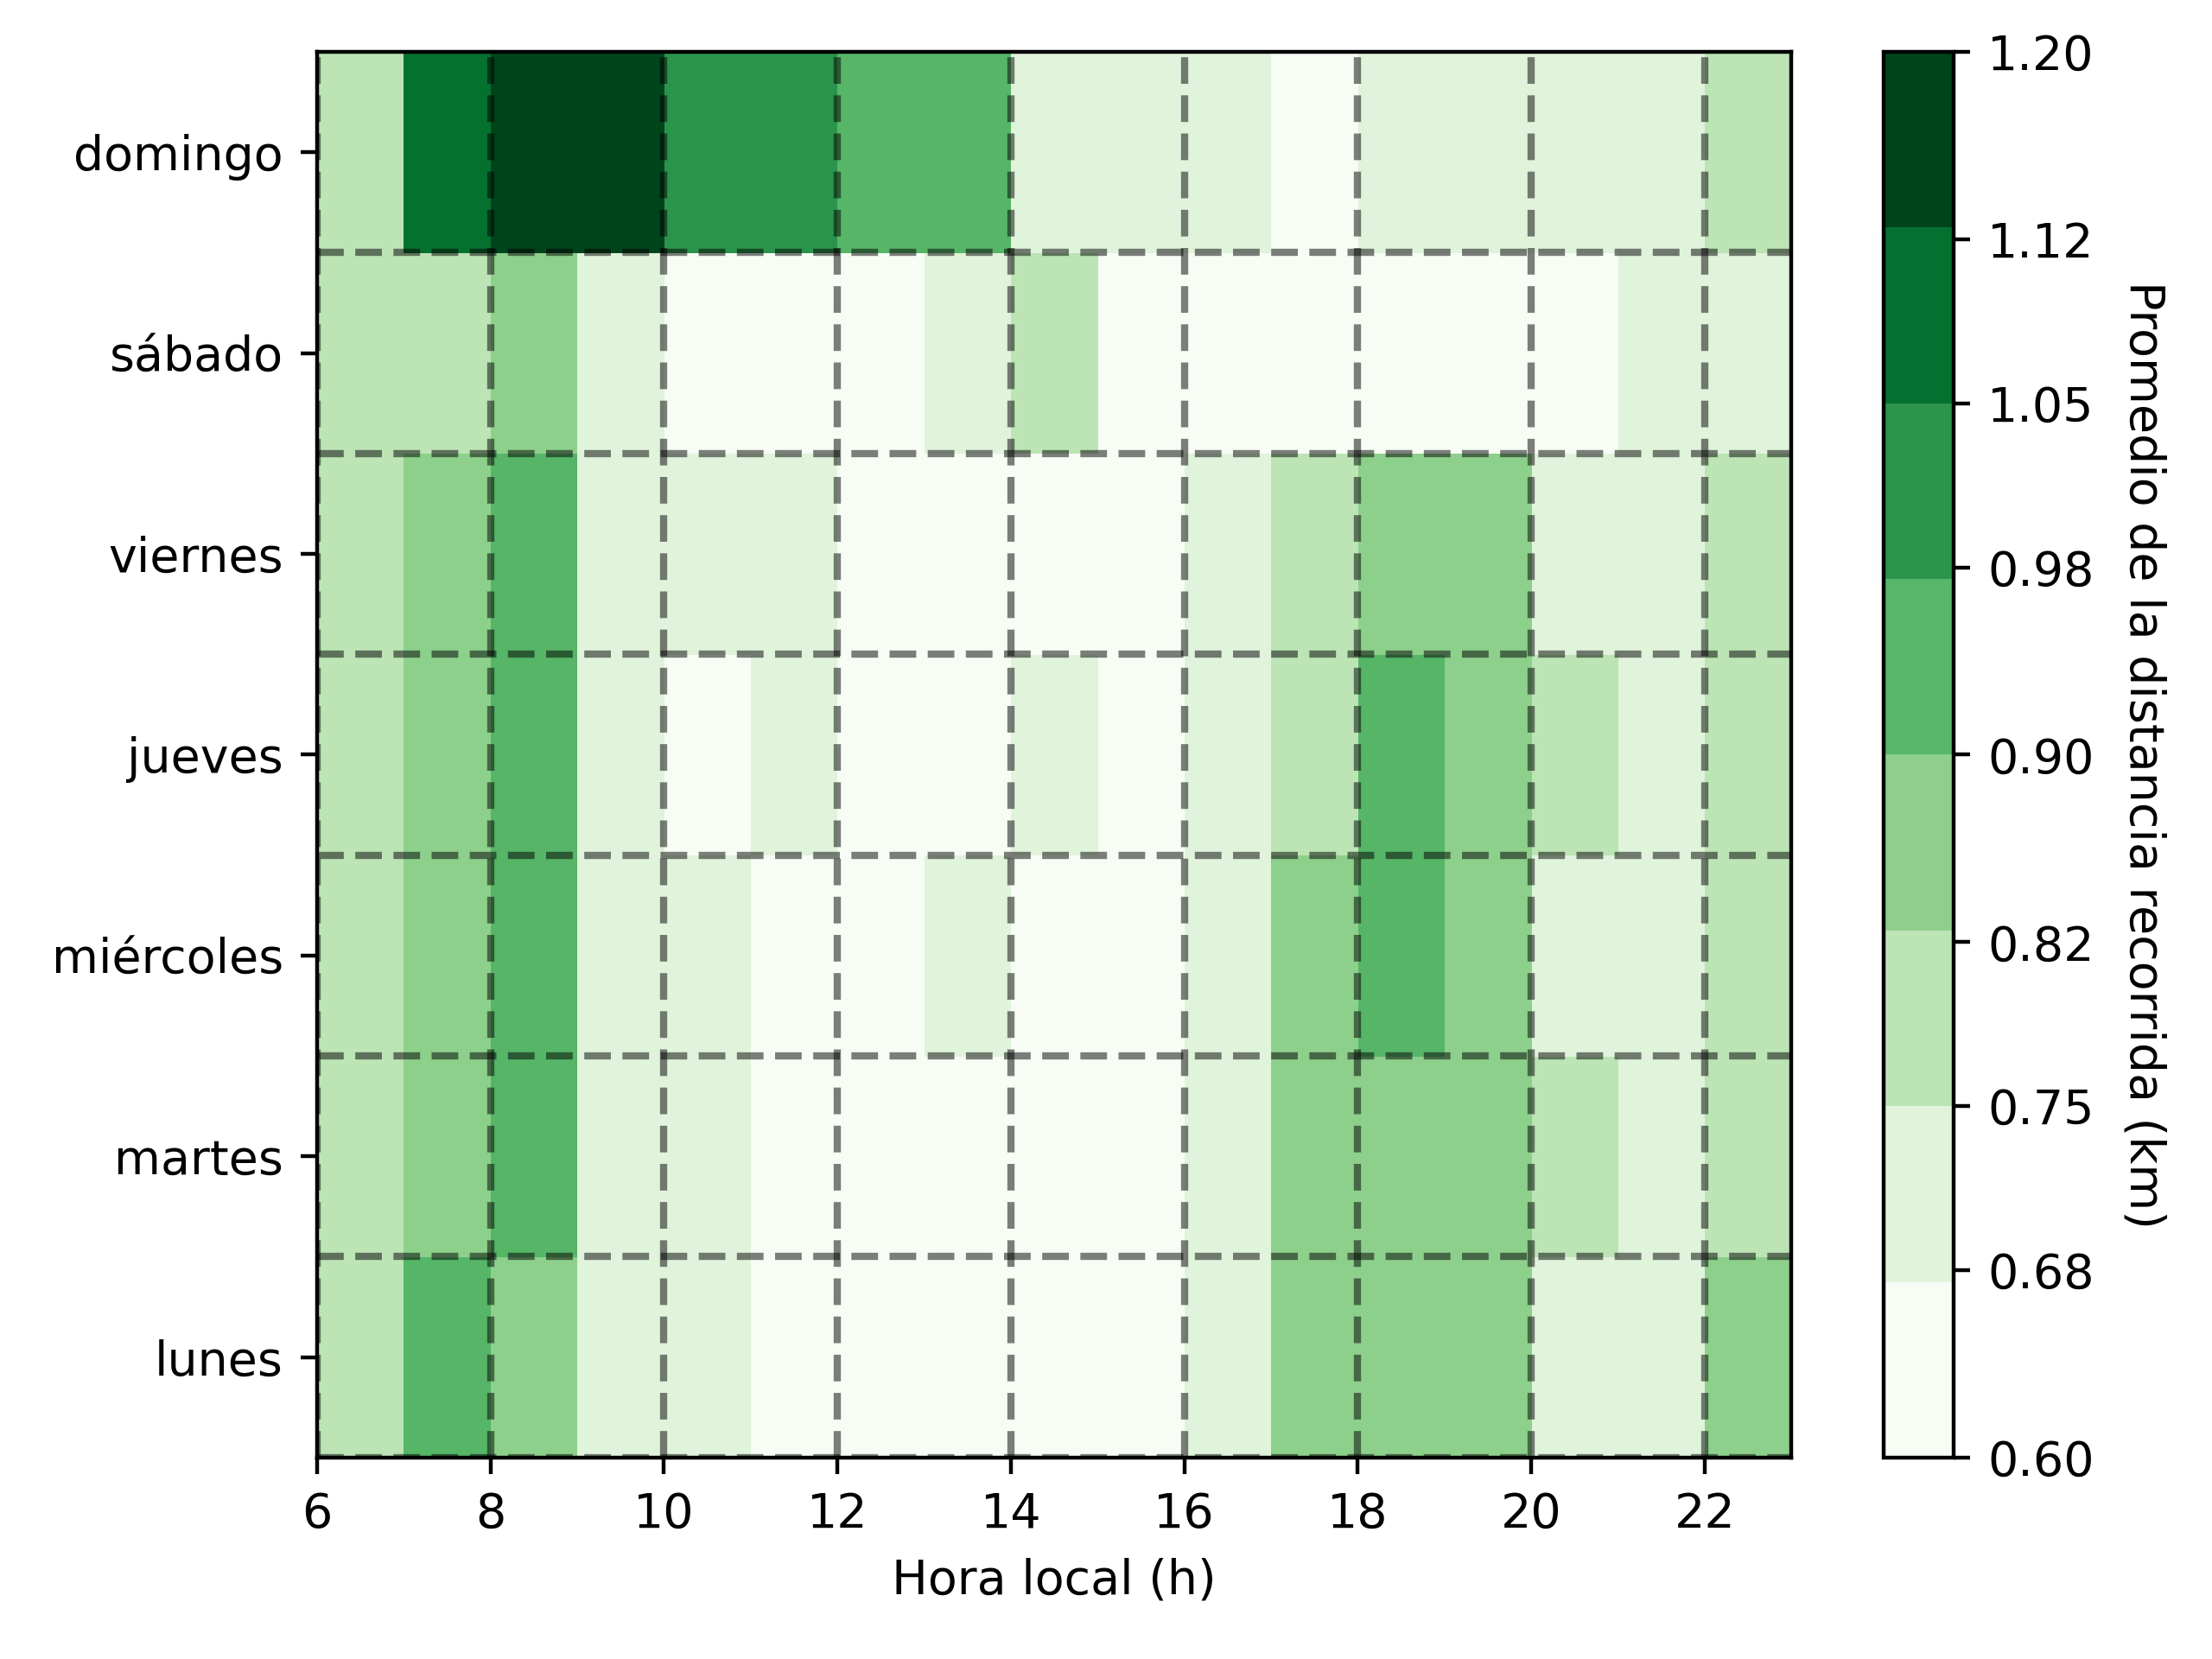
\includegraphics[width=8cm]{Graphics/daily_hourly_mean_distance.png}
        \caption{Promedio diario semanal.}
        \label{fig:daily_hourly_mean_distance}
    \end{subfigure}
    \begin{subfigure}[b]{8cm}
        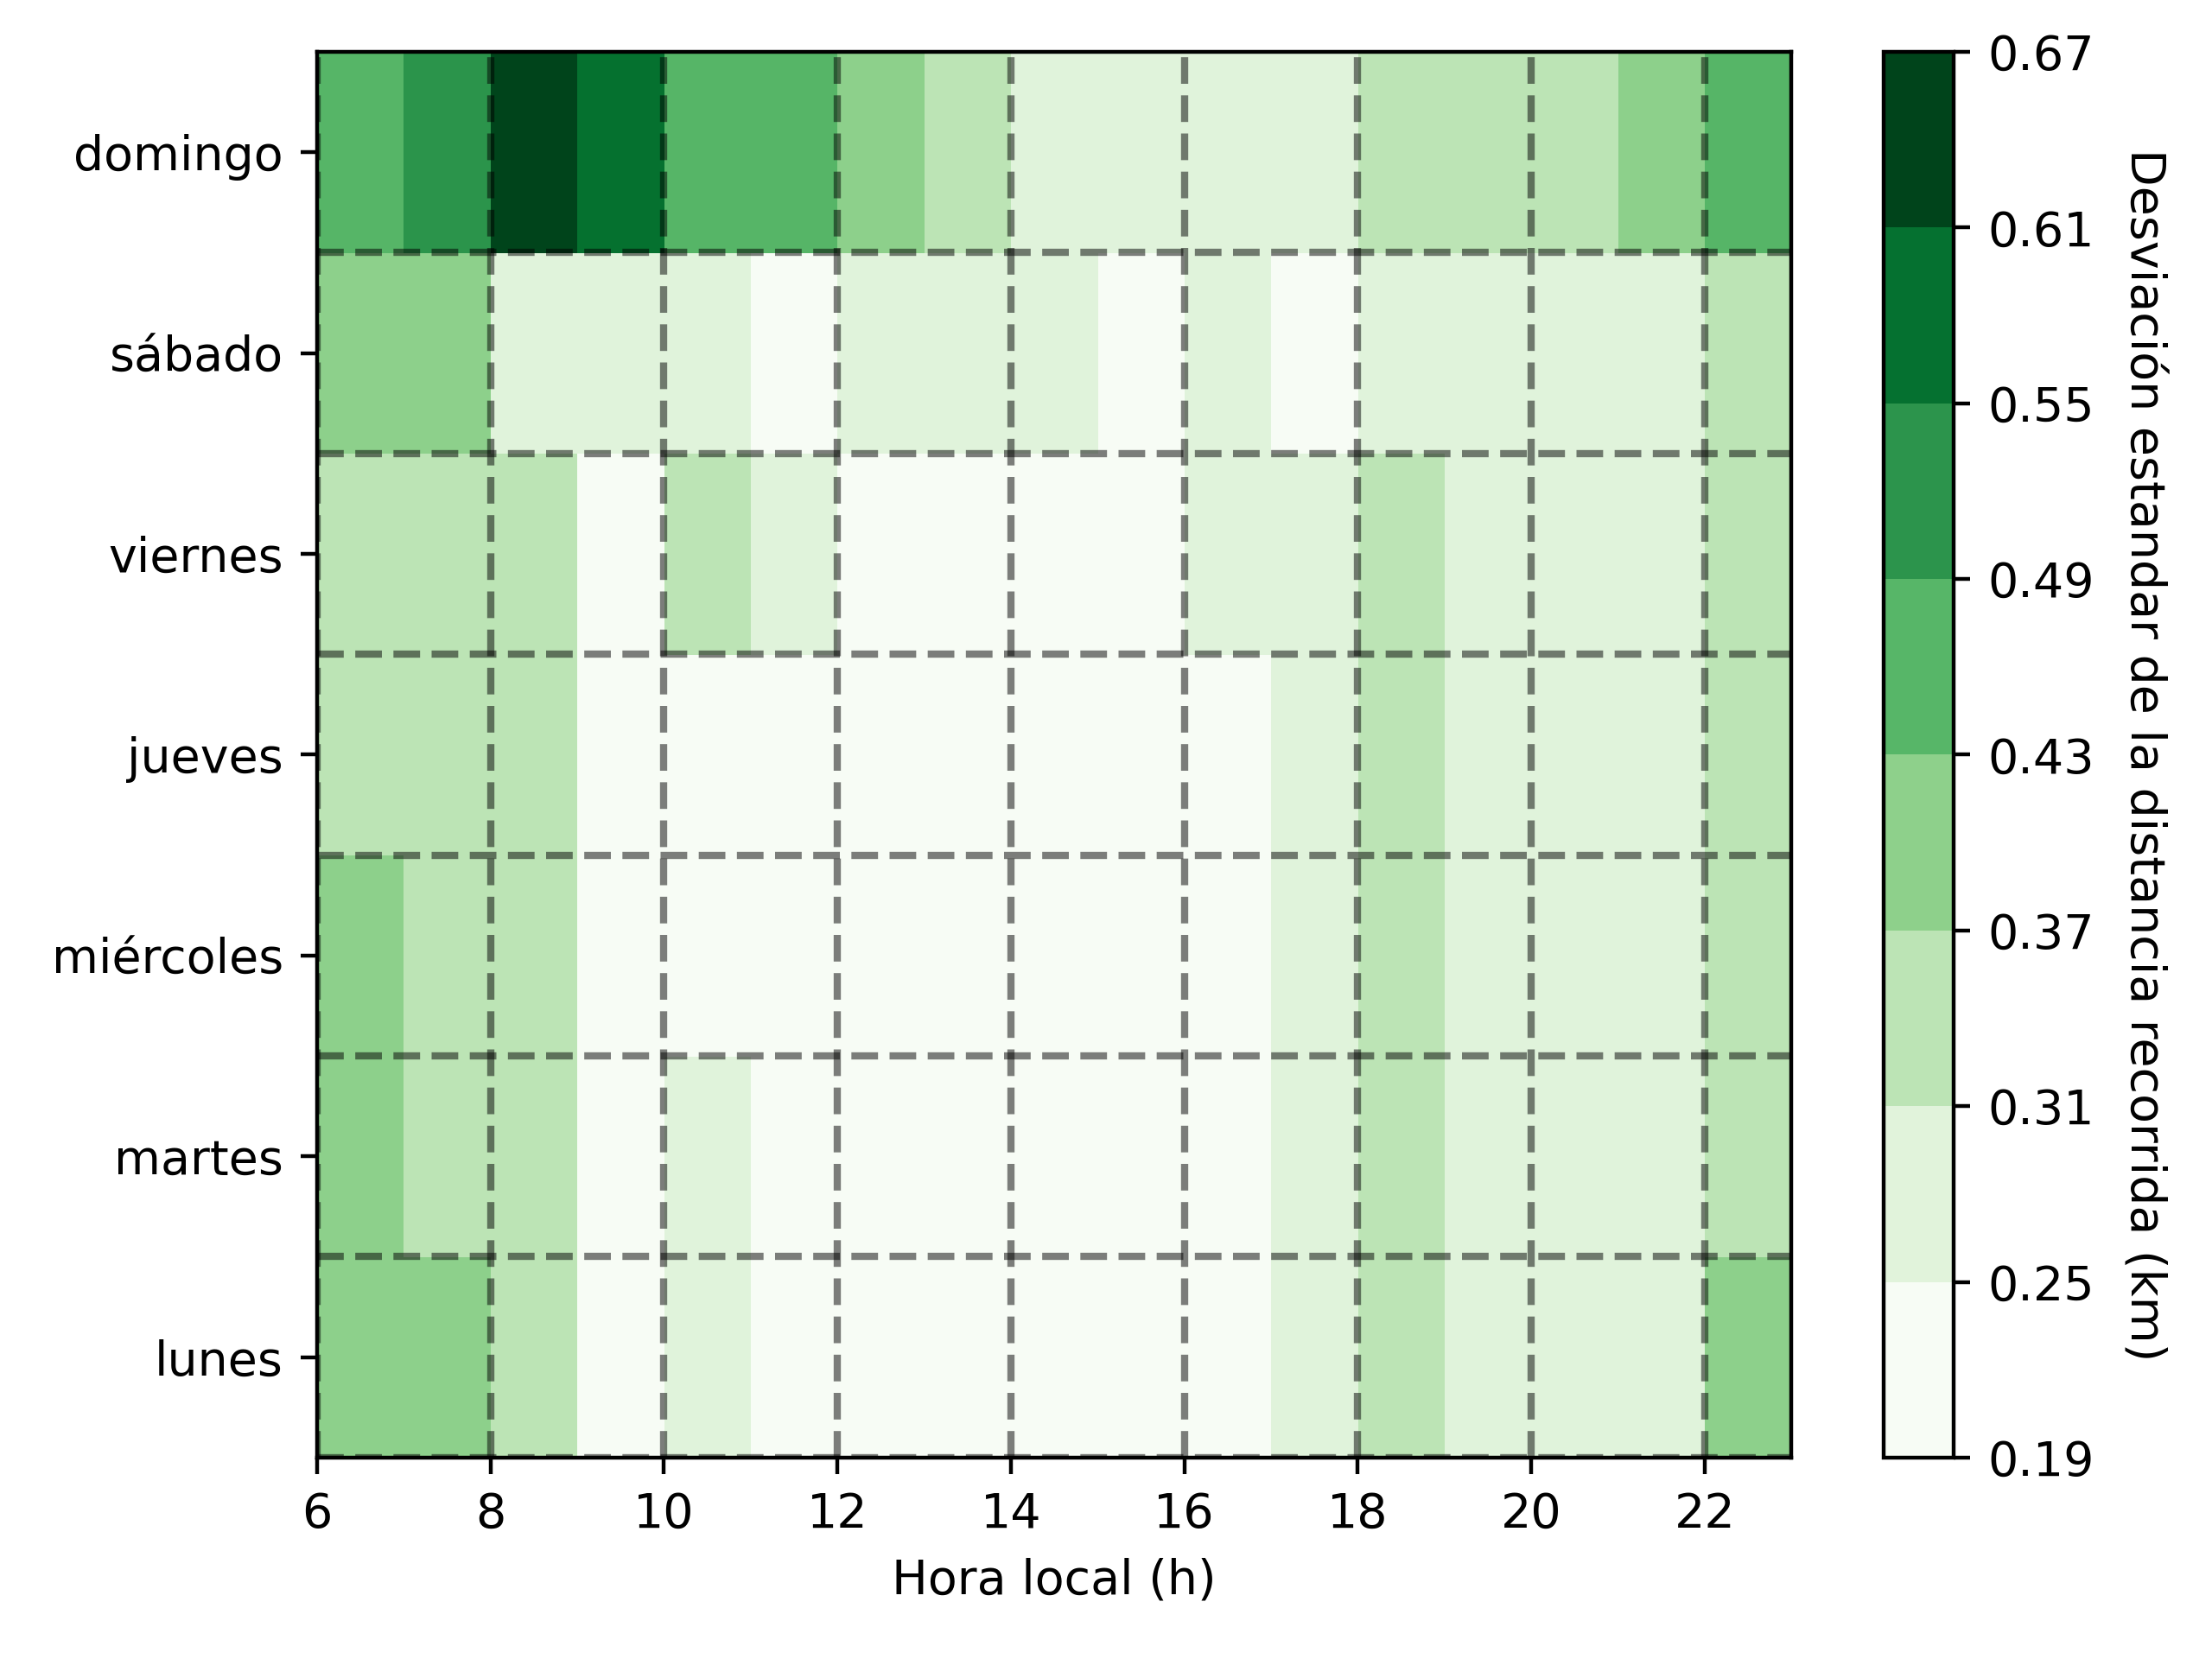
\includegraphics[width=8cm]{Graphics/daily_hourly_var_distance.png}
        \caption{Desviación estandar diaria semanal.}
        \label{fig:daily_hourly_var_distance}
    \end{subfigure}
    \caption{Distancia promedio y desviación estandar diaria semanal por hora recorrida por lo usuarios calculadas con las ecuaciones \ref{eq:daily_hourly_mean} y \ref{eq:daily_hourly_var}.}
    \label{fig:daily_hourly_distance}
\end{figure}

Se presenta en el periodo de las 8 y 10 horas los días domingo, dando indicios que en ese periodo se usan de manera recreativa. Esta suposición también puede ser realizada con la figura \ref{fig:daily_hourly_var_distance}, ya que la variación en ese periodo de tiempo es mayor, y esto puede ser debido a que son usadas en diversas actividades. En cambio entre semana la varianza es poca, dando la impresión que los usuarios realizan una actividad semejante como lo es el transporte de un lugar hacia otro.


\subsubsection{Frecuencia de la distancia recorrida por viaje}

A partir del promedio por hora definido en la ecuación \ref{eq:hourly_mean} se obtuvo la distribución mostrada en la figura \ref{fig:distribution_distances}. Al existir estaciones de origen y destino, las distancias pueden ser tratadas como una variable discreta, ya que solo existe un conjunto finito. Se observa que existen dos máximos en las estaciones utilizadas. Las cuales corresponden a las distancias entre las estaciones más usadas como se mostro en la figuras \ref{fig:distribution_origin} y \ref{fig:distribution_destiny}.

\begin{figure}[H]
    \centering
    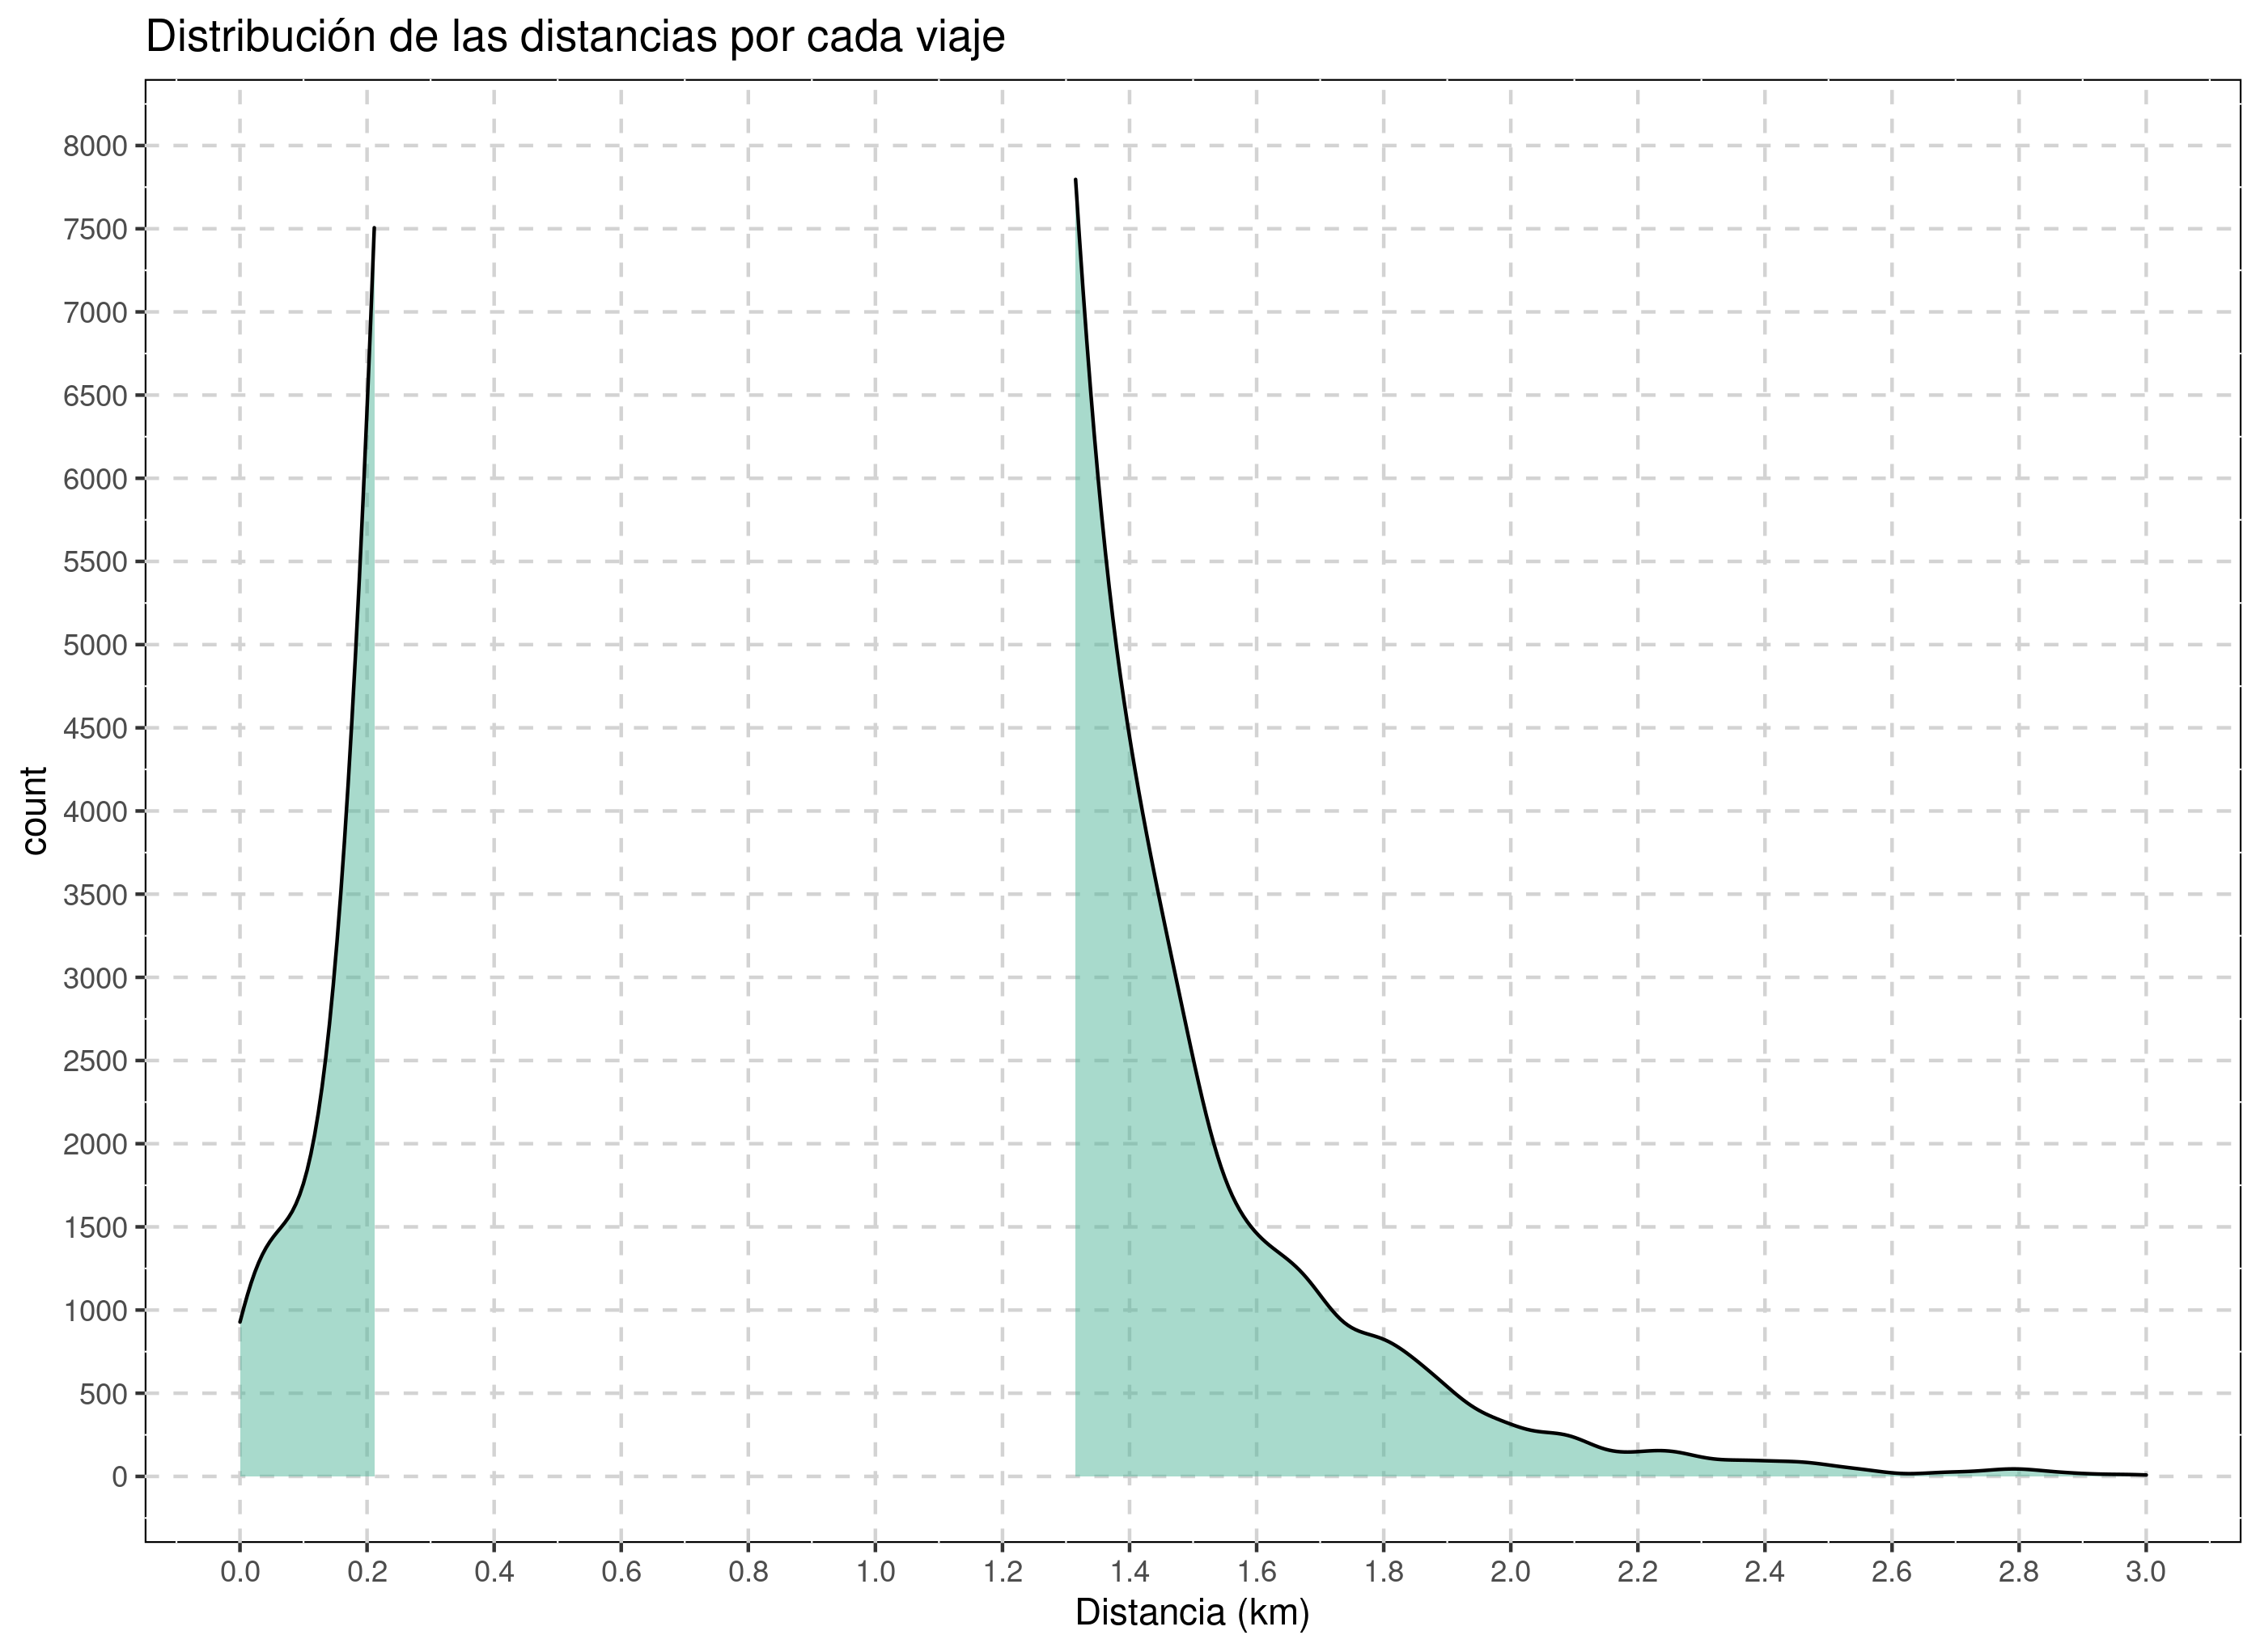
\includegraphics[width=16cm]{Graphics/distribution_distance.png}
    \caption{Frecuencia de las distancias recorridas en el periodo 2015-2018.}
    \label{fig:distribution_distances}
\end{figure}